% Chapter Template

\chapter{Related Work} % Main chapter title

\label{ch:rw} % Change X to a consecutive number; for referencing this chapter elsewhere, use \ref{ChapterX}

\lhead{Chapter \ref{ch:rw}. \emph{Related work}} % Change X to a consecutive number; this is for the header on each page - perhaps a shortened title

%----------------------------------------------------------------------------------------
%	INTRO TEXT
%----------------------------------------------------------------------------------------
The goal of this thesis, to design and implement a \textbf{learning-capable} dialogue system, combines different disciplines within the fields of Artificial Intelligence and Linguistics. This chapter reviews the most relevant work that has been previously done, and that contributed to the realization of this project.

This work includes research on \textbf{sentence similarity} measures (Section \ref{ch:rw:sim}), corpus-based approaches to \textbf{language processing} (Section \ref{ch:rw:ml}), with a particular attention to the IBM Watson structure, that inspired the meaning matching part of the software, and, of course, literature about the Information State Update (\textbf{ISU}) approach to dialogue management (Section \ref{ch:rw:isu}), which constitutes the basic framework of the application we developed.

%----------------------------------------------------------------------------------------
%	SENTENCE SIMILARITY
%----------------------------------------------------------------------------------------

\section{Sentence Similarity} \label{ch:rw:sim}
As it has been mentioned in the previous chapter, the core task of the system is to associate an unknown sentence with its correct meaning, where each meaning is defined by a set of sentences realizing it. Therefore, one of the constituent capabilities that the system must implement is the ability to tell whether two sentences \textbf{share the same meaning} or not.

The problem of scoring the similarity between two sentences is not new in the literature, and a number of different approaches already exist to tackle it. \cite{Achananuparp:2008:ESS:1430555.1430594} suggest to classify the existing measures in \textbf{three categories}: word overlap measures, TF-IDF measures and Linguistic measures. \textbf{Word overlap} scores are computed taking into account only the number of words that are shared between the two input sentences; a basic measure of this kind is the Jaccard coefficient, which is defined as the size of the intersection of the words in the two sentences compared to the size of the union of the words in the two sentences. \cite{Banerjee03extendedgloss} extended the concept to include a special treatment of phrasal $n$-word overlaps, motivated by the fact that they are much rarer than single word ones. \textbf{TF-IDF} measures are based on term frequency-inverse document frequency, hence the name. Those are common measures to express the importance of a term in a document in an  indicized corpus; respectively, they represent the frequency of the term in the document, and the frequency of the term across all documents. TF-IDF can be used to score the similarity between two sentences, for instance, computing the cosine similarity in a vector-space approach. Lastly, \textbf{linguistic} measures are meant to exploit, intuitively, the linguistic information contained in the input sentences. Such information consists of semantic relations between words, and the syntactic structure that connects them. % Various methods exist to ...

The way sentences are compared in \pname takes into account aspects of all these three types of measures, which are combined together in a feature-oriented fashion; the specific algorithm for sentence comparison is described in Chapter \ref{ch:M2}.

%----------------------------------------------------------------------------------------
%	IBM WATSON
%----------------------------------------------------------------------------------------

\section{Machine Learning for Language Processing} \label{ch:rw:ml}
The task of labeling an unknown sentence with its correct meaning can be easily expressed in terms of Machine Learning. In fact, it is a standard supervised \textbf{classification problem} to learn a class' model from examples, and later use that model to label new data points. In this view, a data point is a natural language sentence, and a label is its meaning. 

\subsection{Parsing and Machine Translation}
A great source of inspiration for this work is represented by \textbf{statistic}, corpus-based methods in Computational Linguistics; a significant example comes from The IBM models for Statistical \textbf{Machine Translation} \citep{Brown:1993:MSM:972470.972474}, that first introduced the idea of feeding statistically intensive \textbf{Machine Learning} algorithms with big data from corpora, which nowadays is the dominant paradigm in MT; insightful is also the work on Data Oriented Parsing, and particularly the U-DOP model for \textbf{Unsupervised Language Learning} \citep{Bod:2006:UPU:1596276.1596293}, whose core idea is to initially assume all the possible syntax trees for a set of sentences as equally possible, and then use all the possible sub-trees of them to compute the most probable parse trees, letting the structure of the language emerge from the data.

This work in Computational Linguistics is well reflected in our project, as a strong part of it consists of finding \textbf{alignments} of strings sharing similar meanings. We will see (Chapters \ref{ch:arch} and \ref{ch:M2}) that the computation of these alignments happens in a similar setting as in corpus-based Machine Translation: every alignment is initially considered plausible\footnote{It is worth to note that, where in classic Machine Translation every alignment is initially considered possible with equal probability, here we use some heuristics to provide a clever initialization, in order to cope with the limited amount of training data we have.}, but recurrent ones are reinforced more often, and will thus achieve better and better scores as the model is trained with more examples. Also, the same procedure that computes the alignments is used to let \textbf{syntactic structures} emerge from training data, and from processing new input sentences.

\subsection{IBM Watson} \label{ch:rw:ml:watson}
Particularly inspiring for the development of this thesis was the work done by IBM on Watson. \textbf{IBM Watson} is a question answering computer system that applies advanced Artificial Intelligence techniques to the field of open domain question answering \citep{Ferrucci:2011:IW:2024723.2019525}. That is, a software capable of crawling a database of knowledge looking for an answer to any specific English question given as input; along with the answer, the system outputs also a confidence value, that accurately reflects the probability of the answer being correct. Watson was in the headlines in 2011 for competing in the popular American quiz show \textit{Jeopardy!}, defeating former winners  Brad Rutter and Ken Jennings, and thus winning the \$1 million first prize.

What is interesting about Watson, in connection to our work, is the feature-based approach to \textbf{evidence scoring} that is used to select the correct answers. Figure \ref{ch:rw:ml:watson} \citep{journals/aim/FerrucciBCFGKLMNPSW10} shows a bird-eye view of the whole Watson architecture; the part of this process that is especially interesting for us is the \textit{Hypothesis and evidence scoring}: at that point, the system receives a set of candidate answers for the input question; each of this answers will be run through a series of procedures whose purpose is to find evidence supporting that answer. Most of these procedures are not particularly sophisticate, in fact the clever part of the algorithm is to combine a \textbf{high number of features} to obtain an accurate final score value. This is done by training Watson's hypermodel with data from previous \textit{Jeopardy!} games; the hypermodel consists of a set of weights, that are then used to produce the optimal linear combination of the features.

Even though this latter meta-learning aspect is not implemented in our work, we will find a similar feature-based scoring approach in the core matching algorithm of the Language Unit, discussed in detail in Chapter \ref{ch:M2}.

\begin{figure}
	\centering
	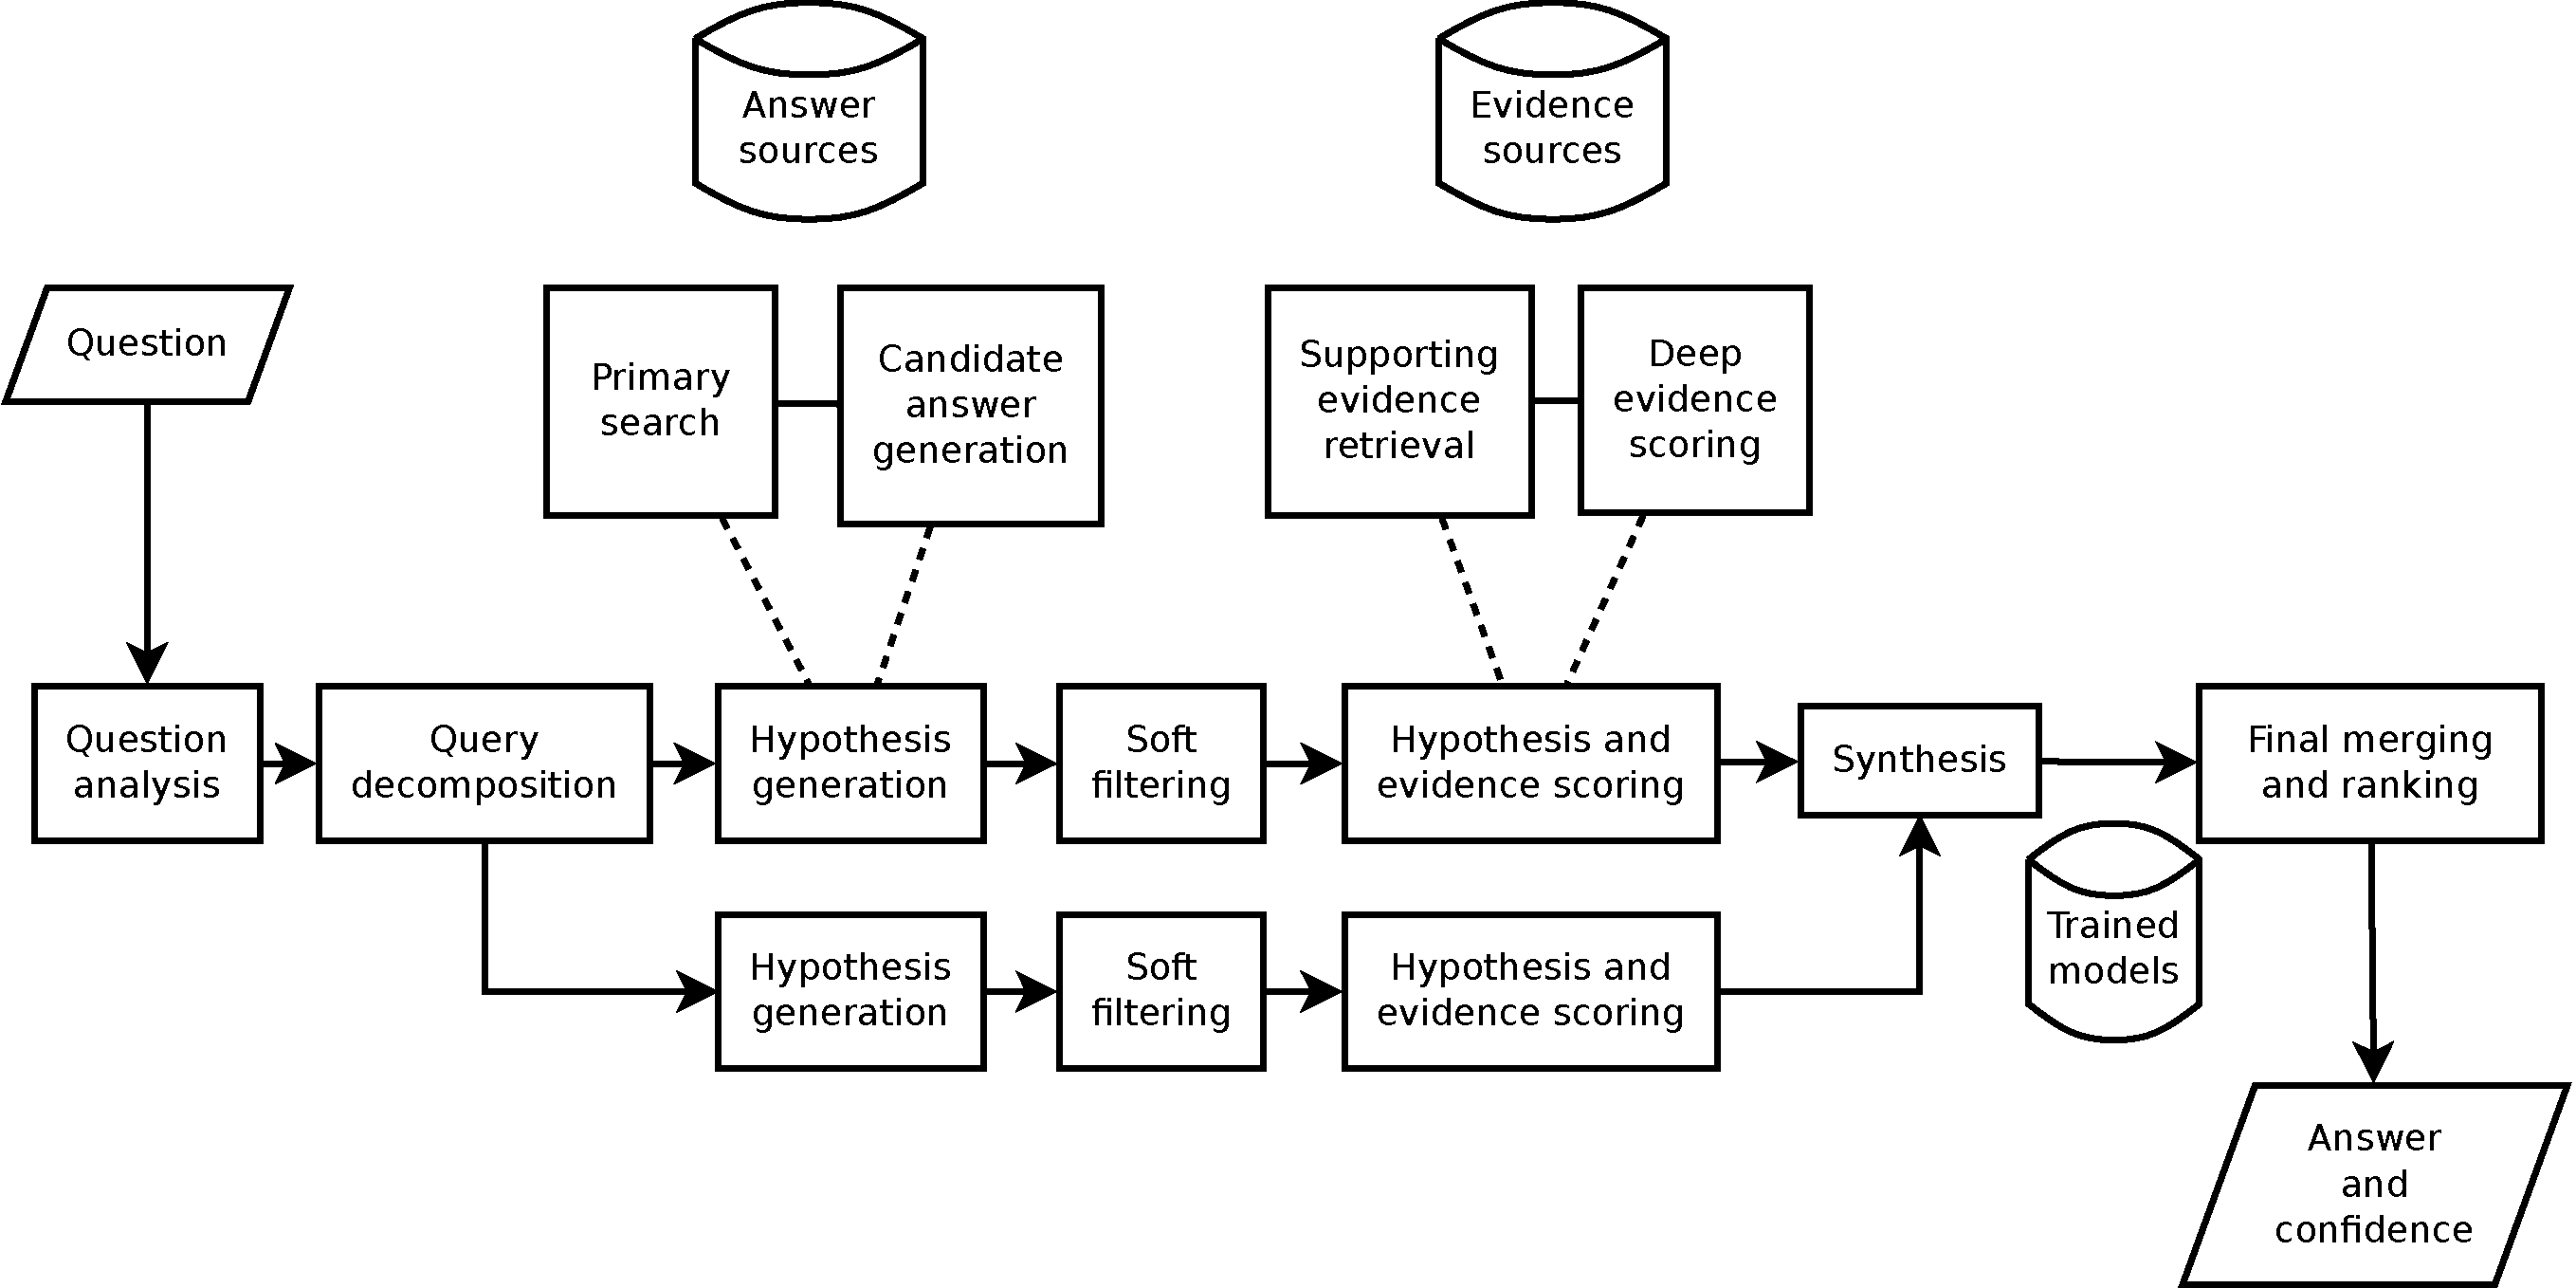
\includegraphics[width=12cm]{Pictures/DeepQA.pdf}
	\caption{Watson's high level architecture}
	\label{ch:rw:ml:watson}
\end{figure}



%----------------------------------------------------------------------------------------
%	DIALOGUE SYSTEMS
%----------------------------------------------------------------------------------------

\section{Dialogue Interaction} \label{ch:rw:isu}

As we have mentioned in Section \ref{ch:introduction:ds}, Dialogue Systems have a long history in the Artificial Intelligence literature. Section \ref{ch:rw:ds:isu} will introduce the Information State Update framework for dialogue management, on which our software is based. Section \ref{ch:rw:ds:grounding} will present some work on grounding and clarification, which was useful to develop the clarification procedures of SVPlay.

\subsection{Information State Update Framework}\label{ch:rw:ds:isu}
The ISU approach to Dialogue Management, as it is described by \cite{TraumLarsson03p325}, can be seen as an attempt to reduce the gap between ``theories of dialogue that linguists or philosophers of language may devise and theories directly implemented in dialogue systems".

The linguistic and philosophical roots of this theory can be found in the notion of \textbf{common ground}, as it is defined by [STALNAKER CITE]; on Stalnaker's account, the common ground consists of an unstrucrured set of all the possible worlds that are compatible with the propositions asserted so far in the dialogue. A slightly more sophisticated formulation of the same concept comes from [LEWIS, CITE], who, drawing a parallel between dialogues and baseball, introduces the notion of ``conversational scoreboard", to keep track of the participants' moves. Even closer to the model of Traum and Larsson is \textbf{Ginzburg's dialogue gameboard} \citep{LLBook59315}; one of the main differences between this model and the other two is represented by the inner structure of the scoreboard, which in Ginzburg is not just a set of propositions, but rather provides a structure made of facts, questions under discussion (QUD) and moves.

Traum and Larsson's notion of \textbf{Information State} (IS) takes Ginzburg's DGB one step further, by extending it with a formal representation of what Ginzburg calls the unpublished part of a dialogue partner's (DP) mental state (UNPUB-MS), and that will become the private part of the Information State. Figure \ref{ch:rw:ds:isu:ibisis} shows a simple Information State type, as it is implemented in the IBiS1 system \citep[p. 36]{Larsson02issue-baseddialogue}. It can be easily noticed that the IS is split in two sections, ``Private" and ``Shared", each of them containing formal representations of informational components: an agenda of actions being executed, a plan for future actions and a set of beliefs for the \textbf{private} part, the set of propositions in the common ground, a stack of questions under discussion, and the last utterance in the \textbf{shared} part.

Besides the notion of IS, the ISU framework includes two \textbf{additional components}: a set of dialogue moves and a set of update rules.

The central concept of ISU-based systems is to \textbf{update} this, initially empty, Information State, according to the dialogue moves performed by the DPs. A \textbf{dialogue move} is tipycally the formal interpretation of a natural language utterance (e.g.\ the English sentence ``What's your name?" can be interpreted as the dialogue move ``\texttt{ask(?X.my\_name(X))}"\footnote{Let's not enter the detail of the $\lambda$-calculus-like representation of the user move: what is important is that it is expressed in a form that the system can work with.}), but, in more complex systems, can be also derived from a different type of interaction (e.g.\ a gesture). The system receives this moves, and is able to modify the IS accordingly (e.g.\ inserting a new question under discussion, or marking an action as completed, and so on), by running them through a set of \textbf{update rules}, and an \textbf{update strategy}, to decide on which rules to apply when more than one can be selected.

\begin{figure}
	\centering
	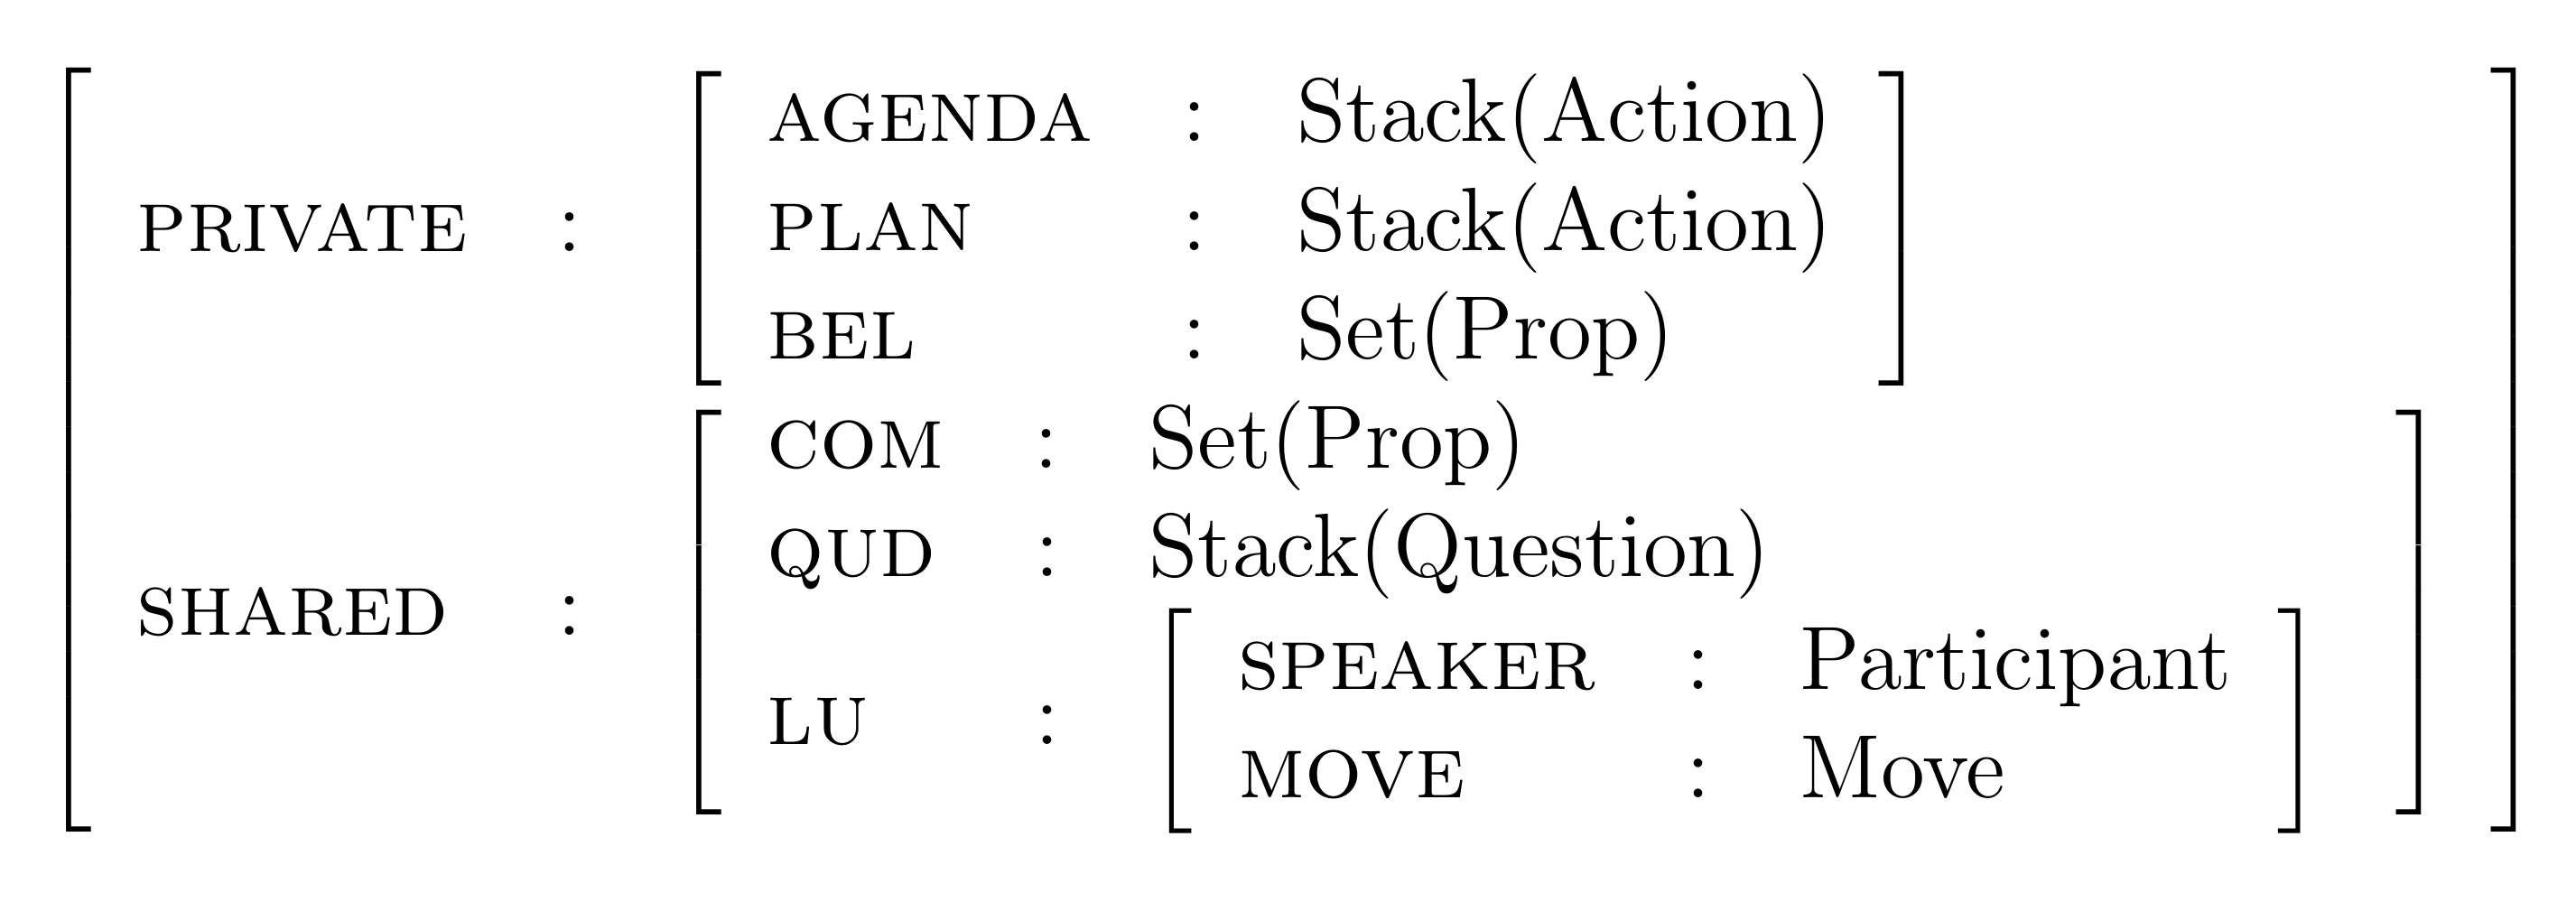
\includegraphics{Pictures/ibis1_is.png}
	\caption{Information State, as it is implemented in IBiS1}
	\label{ch:rw:ds:isu:ibisis}
\end{figure}

This work is relevant to us, as our software builds on the TDM dialogue management library (see Section \ref{ch:arch:TDM}), which implements the Information State Update framework. Our contribution is located at the \textbf{interpretation} level, that is, the part which is resposible of receiving the user utterance and converting into a formally defined dialogue move. Particularly, we will extend the existing library with a new interpretation module, that is able to perform fuzzy matching of natural language sentences, and implements an \textbf{interactive learning} procedure to exploit the information contained in unknown examples. Once the sentences have been interpreted, standard dialogue moves are returned, to be used in the system as it would happen with the previous version of the interpretation module.

\subsection{Grounding and clarification}\label{ch:rw:ds:grounding}
Herbert Clark in \cite{clark_1996} points out how, in the nature of human dialogue interaction, a major role is played by a social component, the activities that, alongside the individual communicative intentions, ensure the coordination between dialogue partners. In particular, \textbf{grounding} is the act of enstablishing mutual knowledge among the participants. \cite{Gabsdil03clarificationin} points out how this process, while being almost effortless for human speakers, represents a challenge in computer dialogue systems, and argues for the importance of having as natural grounding interactions as possible.

The following example, taken from Gabsdil's paper, shows a grounding act, in the form of a \textbf{clarification question} by one of the DPs:
\begin{verbatim}
A: You turn the second road on your left hand side
B: You mean Marchmont Road?
\end{verbatim}
B wants to make sure that both A and himself are talking about the same road: this necessity for clarification may be due to \textbf{different reasons}, for instance A might have provided an inaccurate description of his intention, or B might haven't heard correctly A's utterance. Clark identifies \textbf{four levels} speaker and listener have to be coordinated on in dialogue: level 1, where participants \textbf{enstablish} communication by respectively executing and attending to the communicative behaviour; level 2, where A presents a \textbf{signal} to B, and B identifies it; level 3, where B recognises the \textbf{meaning} of A's signal; level 4, where A proposes a \textbf{joint project} to B, and B considers it.

Our software will be especially concerned with Clark's \textbf{third level}, as the user signal, given in the form of written utterances, is assumed to be considered and recognised correctly by the system\footnote{The actual implementation of our software allows the replacement of the text input module with a Speech Recognition one; in this case, uncertainty at level 2 is introduced. This case however is not covered in this thesis.} \footnote{Yet the occurrence of typographical errors is possible. This case can also be located at meaning level, as the signal is still conveyed faithfully from the user to the system.}. It is worth to point out that the software's pragmatic interpretation of the user utterances has a 1:1 correlation with their semantic representation (e.g.\ the sentence ``Increase the volume" is labeled as ``\texttt{request(increase\_volume)}", a label that direclty expresses the intended meaning of the user, that is, assigning to the system the task to increase the volume), therefore levels 3 and 4 de facto collapse into a single one.

One more notion that has been used in our work is Gabsdil's classification of different types of \textbf{non-understanding} into cases where no interpretation is available, cases of uncertain interpretation (one interpretation is still available), and cases of ambiguous interpretation (two or more alternatives are available). We will draw on the same classification in Section \ref{ch:interaction:mmw}, where we will describe how the software deals with utterances that have not been understood. In particular, we will see that the ``no interepretation" case will be answered with a rephrase request, whereas the other two will be solved with a single polar question\footnote{Note that, as Gabsdil also says, the most appropriate way to answer a case of ambiguous interpretation would be with a wh-question; as it will be explained better in Chapter \ref{ch:interaction}, this has not been done mainly for technical reasons.}.

Lastly, Gabsdil also argues for \textbf{partial clarification questions}, being clarification request that are targeted to an especially misunderstood part of the user utterance. As an example, in the context of music player application, let's consider the dialogue:
\begin{verbatim}
U: Put on my favourite from Zappa
S: I don't understand, can you repeat?
\end{verbatim}
In this case the system's clarification question is generic, and doesn't sound as natural as the one in the following example:
\begin{verbatim}
U: Put on my favourite from Zappa
S: You mean `Sheik Yerbouti'?
\end{verbatim}
Gabsdil points out how a particular effort is required to implement this type of questions. We will address partial clarification questions in Chapter \ref{ch:interaction}.

\section{Summary}
In this chapter we have reviewed some of the most relevant work that inspired our project.

We looked at \textbf{sentence similarity} measures, they are central for our application, as its core meaning matching features relies on the comparison and scoring of the input sentences against existing examples. According to the literature, we perform such comparison taking into account word overlapping, term frequency and linguistic features.

Great inspiration also came from the field of \textbf{machine learning}, and particularly from its applications in computational linguistics. We find the same data-driven approach, that is, letting structures and alignments emerge from examples, in statistic machine translation and parsing. Especially relevant has been the work of IBM on Watson, because of its feature-based scoring approach, that inspired ours.

Finally, research in the field of \textbf{dialogue systems} has to be mentioned, as the software we developed is a dialogue system. In particular, we worked with TDM, a dialogue management library that implements the Information State Update framework. We extended this library with grounding and clarification capabilities (other than with the meaning matching features), that are well present in the literature, both from a philosophical/linguistic perspective and from a computational one.